\chapter{Conclusão}

\section{Trabalhos Futuros}
Tendo como base o que foi realizado neste trabalho, percebe-se que é possível aprimorar o sistema construído acrescentando algumas funcionalizades a mais:
\begin{itemize}
    \item Envio de dados em tempo real para a central;
    \item Utilização do bando de dados HDF;
    \item Criação de \textit{managers} para extrair mensagens não enviadas para o servidor;
    \item Permitir registro de transdutores para cada campus da Universidade;
    \item Calcular médias mensais, semanais e diárias utilizando os pacotes \textit{numpy} e {pandas}.
\end{itemize}

\section{Cronograma}
\begin{figure}[!htpb]
    \centering
    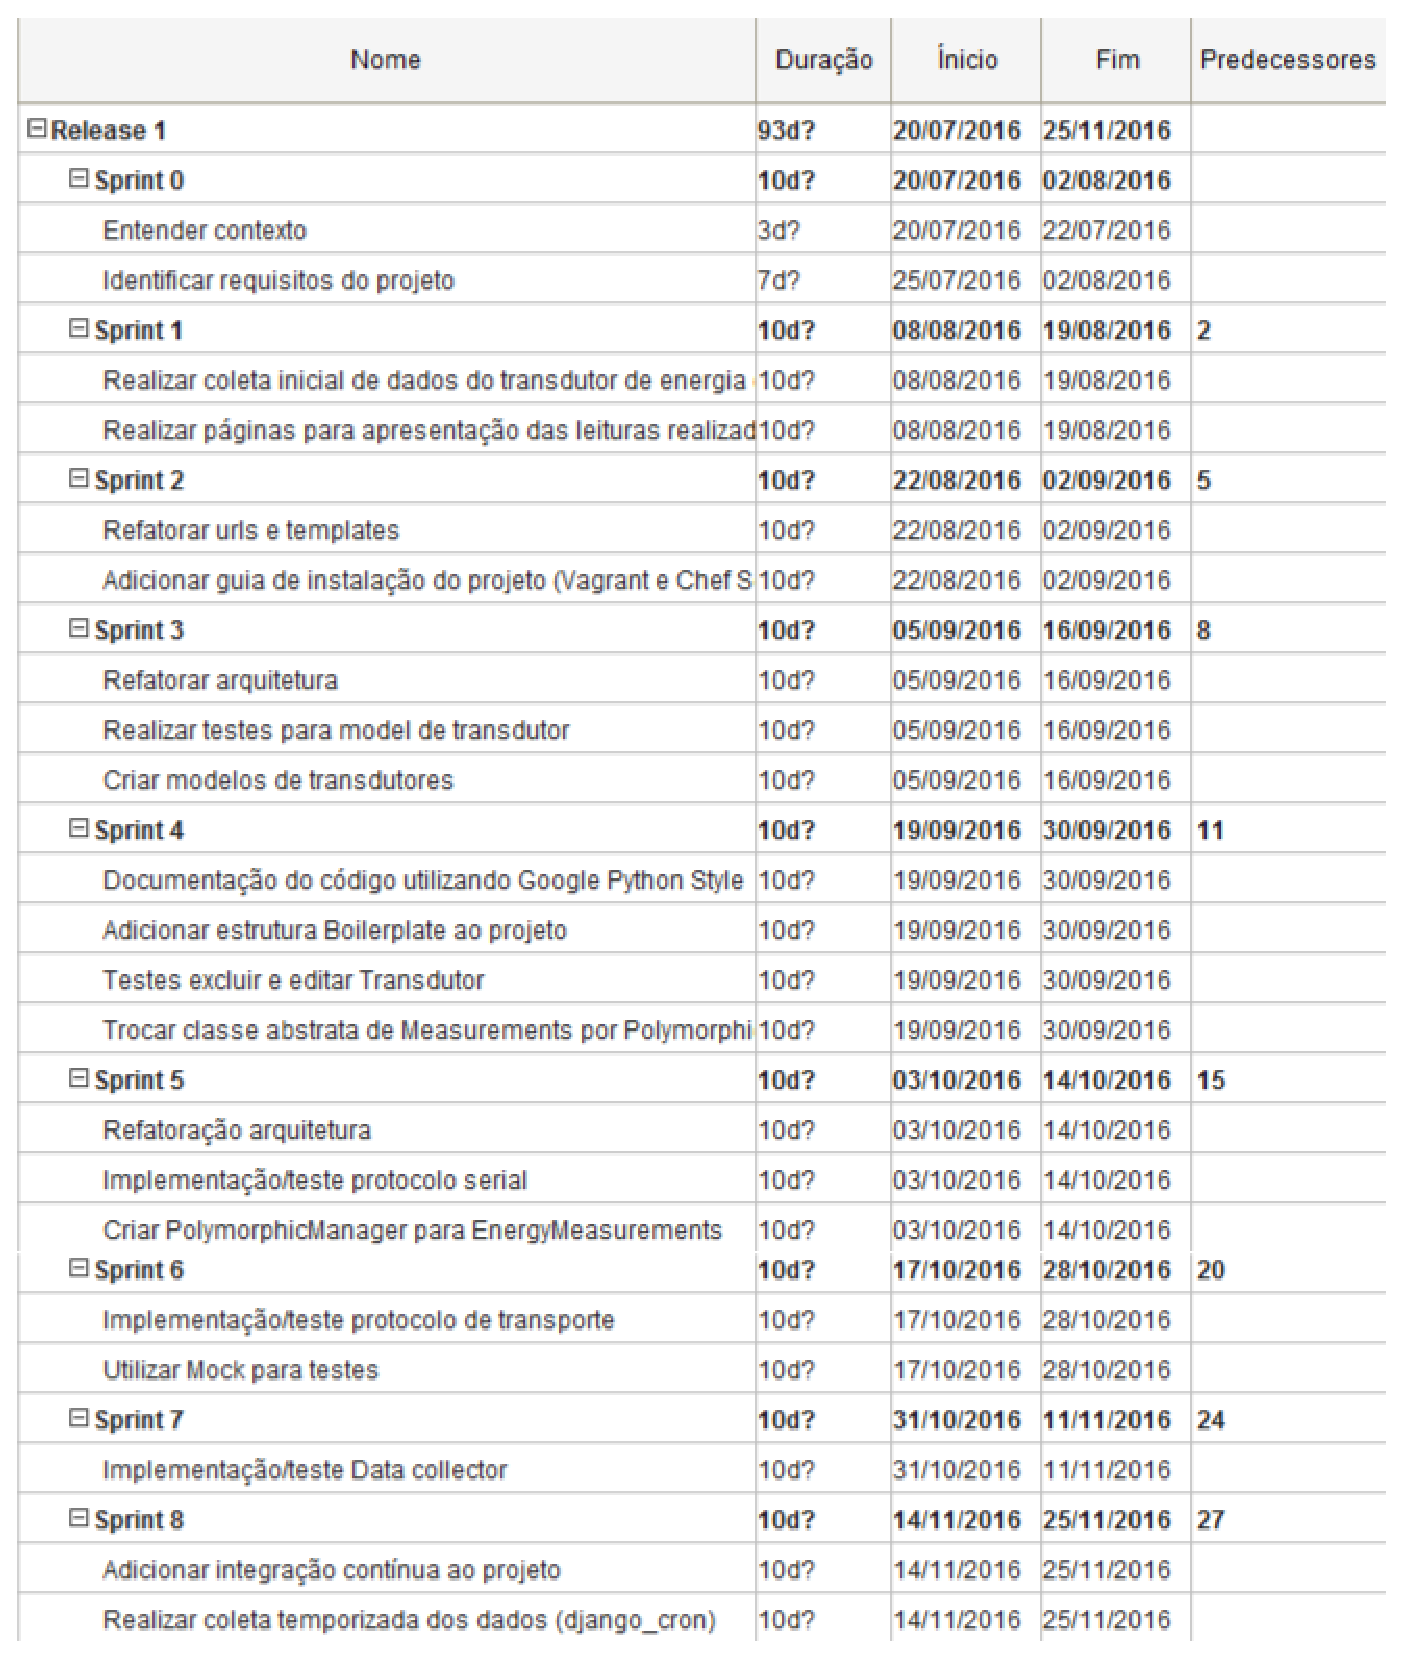
\includegraphics[keepaspectratio=true,scale=0.5]{figuras/cronograma.eps}
    \caption{Cronograma do Projeto. Fonte: autor}
    \label{cronograma}
\end{figure}